\documentclass[9pt]{beamer}
\usepackage[utf8]{inputenc}
\usepackage[T1]{fontenc}
\usepackage[english]{babel}
\usepackage{xcolor}
\usepackage{csquotes}
\newcommand{\highlight}[1]{\colorbox{yellow}{#1}}
\usepackage{expl3}
\usepackage[style=numeric, sorting=none]{biblatex}   % Using biblatex with unsrt style
\addbibresource{bib.bib}  % Add your .bib file here
\usepackage{xcolor}
\definecolor{ForestGreen}{RGB}{34,139,34}  % same shade
\usepackage{booktabs}
\usepackage{amsmath}  % Added this package for better math formatting
\usetheme[
  workplace=mu,
]{MU}

\title[Group Relative Policy Optimization]{Group Relative Policy Optimization}
\author[H. Adamove]{Hugo Adamove\texorpdfstring{\\}{, }}
\institute[MU]{IV125 Formela lab seminar}
\date{\today}
\subject{Presentation Subject}
\keywords{the, presentation, keywords}

\begin{document}

\frame{\titlepage}

\begin{frame}{Topics}
  \begin{itemize}
    \item Recap: RL Framework for LLMs
    \vspace{1em}
    \item From PPO to GRPO
    \vspace{1em}
    \item DeepSeekMath
    \vspace{1em}
    \item DeepSeek-R1
    \end{itemize}
\end{frame}


\begin{frame}{RL Framework for LLMs (consistent notation)}
  \begin{itemize}
    \item \textbf{State} 
          \(s_t = (q,\;o_{<t})\): the query $q$ together with already generated tokens $o_{<t}$.

    \item \textbf{Action $o_t$:} 
          single next token predicted by the LLM.

    \item \textbf{Policy $\pi_\theta$:} 
          per-token distribution  
          \(\pi_\theta(o_t \mid q, o_{<t})\).  
          Probability of a full answer  
          \[
              \pi_\theta(o \mid q)=
              \prod_{t=1}^{|o|} \pi_\theta(o_t \mid q, o_{<t}).
          \]

    \pause
    \item \textbf{Reward $R(q,o)$:} 
          scalar score emitted after the full answer  \begin{itemize}
          \item obtained from a trained Reward model or rule-based Reward functions.
\end{itemize}
    \vfill

    \pause
    \item \textbf{Objective:}  
          maximize expected reward over the question distribution $P(Q)$:
          \[
             J(\theta)=
             \mathbb{E}_{q\sim\mathcal P(Q),\;o\sim\pi_\theta(\cdot\mid q)}
             \bigl[R(q,o)\bigr].
          \]
  \end{itemize}
\end{frame}


\begin{frame}{PPO for LLM Fine-Tuning I}
  \begin{block}{PPO surrogate objective for LLMs}
  The PPO surrogate objective for LLMs can be written as:
  \begin{equation}
    J_{\text{PPO}}(\theta) = \mathbb{E}_{\substack{q \sim P(Q), \\ o \sim \pi_{\theta_{old}}(o|q)}} \left[ \frac{1}{|o|} \sum_{t=1}^{|o|} \min \left( A_t \rho_{t}, A_t \text{clip}(\rho_{t}, 1-\epsilon, 1+\epsilon) \right) \right]
    \label{eq:ppo_rho}
  \end{equation}
  where the probability ratio $\rho_{t}$ under current policy $\pi_{\theta}$ and old policy $\pi_{\theta_{old}}$ is defined as:
  \begin{equation}
    \rho_{t} = \frac{\pi_\theta(o_t|q, o_{<t})}{\pi_{\theta_{old}}(o_t|q, o_{<t})}
    \label{eq:rho_def}
  \end{equation}
  \end{block}
  \vspace{1em} % Add some vertical space

  \begin{itemize}
    \item $A_t$: Estimated advantage at token $o_t$ (next slide).
  \end{itemize}
\end{frame}


\begin{frame}{PPO for LLM Fine-Tuning II — Advantage Estimation}

  \begin{block}{(MC) Advantage Estimation}
  \begin{equation}
      A_t \;=\; r_t \;-\; V_\psi\bigl(q,\,o_{<t}\bigr)
      \label{eq:mc_adv_est}
  \end{equation}
    \vspace{-0.2em}
    \begin{itemize}\setlength\itemsep{0.2em}
      \item $V_\psi$ is a value model trained with an MSE loss  
            $\mathcal{L}_V = \tfrac12\bigl(V_\psi(q,o_{<t}) - R(q,o)\bigr)^2$.
      \item In practice, Generalized Advantage Estimation (GAE) \cite{schulman2015} is also often used.
    \end{itemize}
  \end{block}

  \vspace{0.4em}

\pause
  \begin{block}{Reward with divergence penalty}
  \begin{equation}
      r_t \;=\; R_\varphi\bigl(q,\,o_{\le t}\bigr)
             \;-\; \beta\,\log\frac{\pi_\theta(o_t\mid q,o_{<t})}{\pi_{\text{ref}}(o_t\mid q,o_{<t})}
             \label{eq:reward_ppo}
  \end{equation}
    \vspace{-0.2em}
    \begin{itemize}\setlength\itemsep{0.2em}
      \item $R_\varphi$ — pretrained reward model scoring the (sub-)sequence.
      \item $\pi_{\text{ref}}$ — frozen reference policy (e.g.\ the SFT model before applying RL).
      \item $\beta$ — \textit{KL-coefficient}: penalizes divergence from $\pi_{\text{ref}}$.
    \end{itemize}
  \end{block}

\end{frame}


\begin{frame}{PPO for LLM Fine-Tuning III - "Big Picture"}
  \begin{figure}
    \centering
    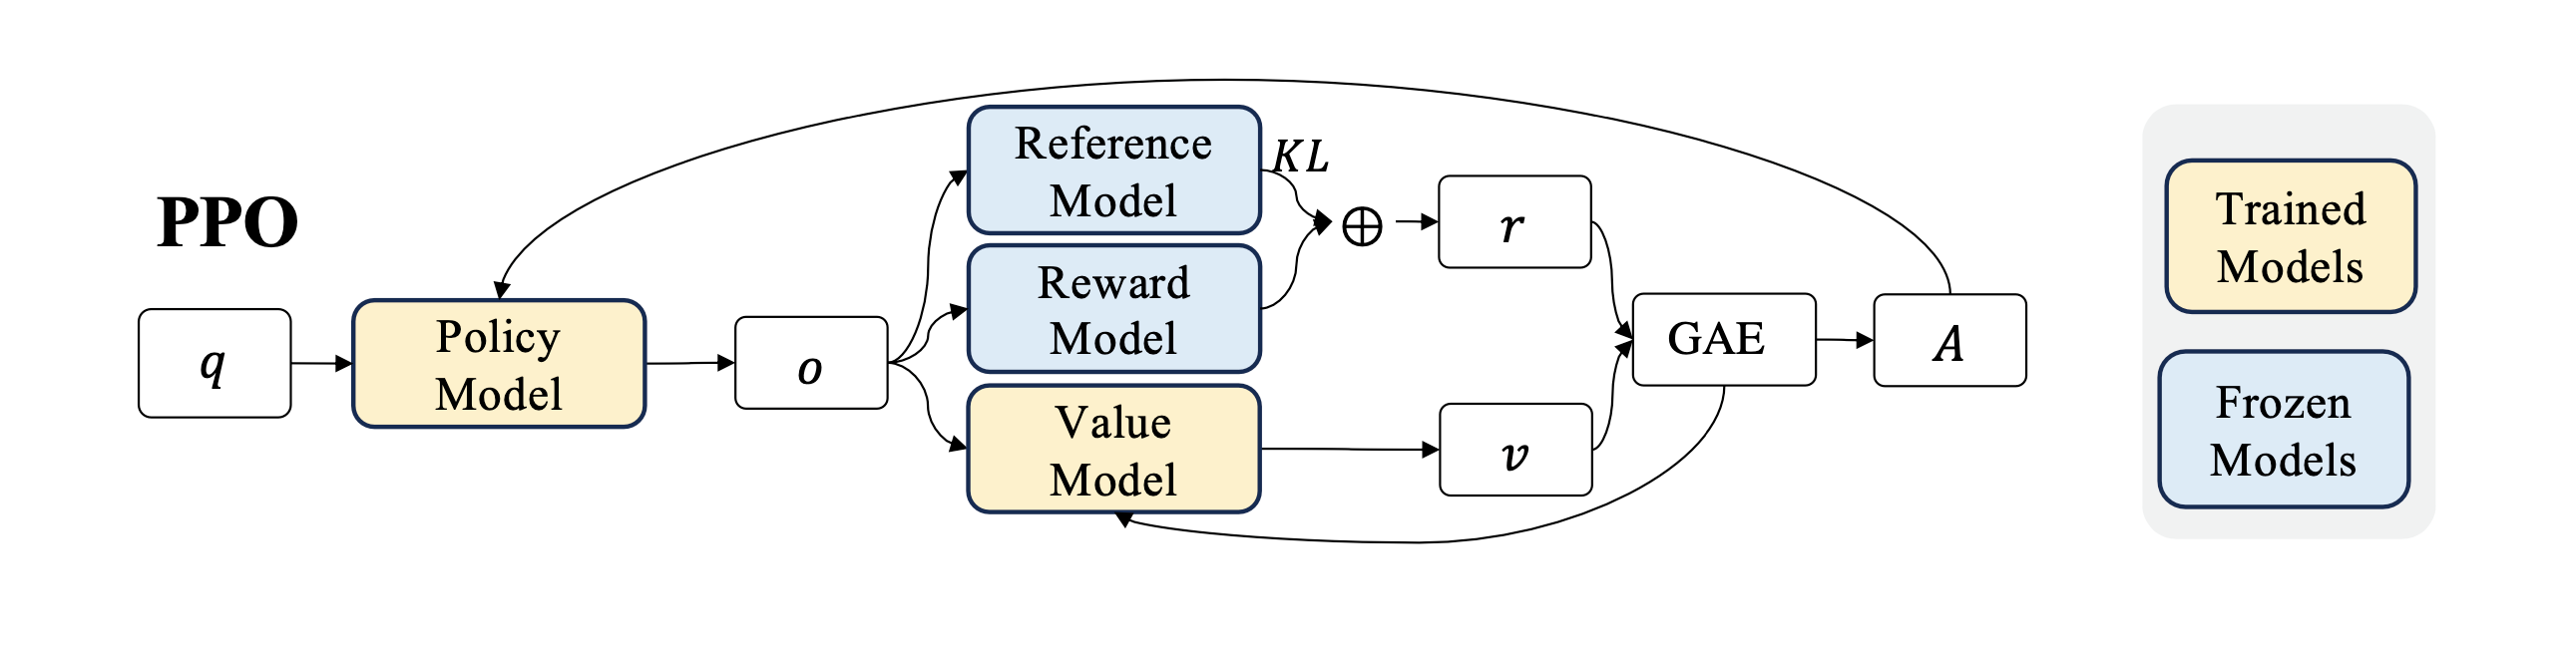
\includegraphics[width=1.0\textwidth]{figures/ppo_big.png}
    \caption{PPO diagram from \cite{shao2024deepseekmathpushinglimitsmathematical}.}
    \label{fig:trl1}
  \end{figure}

  \begin{itemize}
    \item $\pi_{\text{ref}}$ - Reference Model
    \item $R_\varphi$ - Reward Model
    \item $V_\psi$ - Value Model
  \end{itemize}
\end{frame}

%----------------------------------------------------
%–––––––––– Slide 1 ––––––––––%
\begin{frame}{Group Relative Policy Optimization (GRPO)}
  \begin{block}{GRPO surrogate objective}
\begin{equation}
\begin{aligned}
J_{\text{GRPO}}(\theta)=
\mathbb{E}_{\substack{q\sim P(Q),\\
            \textcolor{ForestGreen}{\{o_i\}_{1}^{G}}\sim\pi_{\theta_{\text{old}}}(\cdot|q)}}\Biggl[
\textcolor{ForestGreen}{\frac{1}{G}\sum_{i=1}^{G}}
\frac{1}{|o_i|}\sum_{t=1}^{|o_i|}
&\min\Bigl(\textcolor{blue}{\hat{A}_{i,t}}\;\rho_{i,t},
            \mathrm{clip}(\textcolor{blue}{\hat{A}_{i,t}}\;\rho_{i,t},1-\varepsilon,1+\varepsilon)\Bigr)
\\[0.3em]
&-\;\textcolor{orange}{\beta\,D_{KL}\bigl(\pi_\theta\;\Vert\;\pi_{\text{ref}}\bigr)}
\Biggr],
\label{eq:grpo_obj}
\end{aligned}
\end{equation}
\end{block}

  \vspace{0.3em}

  \textbf{How GRPO differs from PPO}
  \pause
  \begin{itemize}\setlength\itemsep{0.25em}
    \item \textbf{Advantage function}: \textcolor{blue}{$\hat A_{i,t}$} is computed relatively within a
          group of \(G\) sampled answers, we no longer need $V_\psi$ (next slide).
    \pause
    \item \textbf{KL regularisation}: \textcolor{orange}{KL term} is added directly to the loss
          instead of being folded into the reward via \(r_t\).
  \end{itemize}
\end{frame}

%–––––––––– Slide 2 ––––––––––%
\begin{frame}{GRPO – Group-Relative Advantage $\hat{A}_{i,t}$}
  \begin{itemize}\setlength\itemsep{0.4em}

    \item For each question $q$, GRPO samples a group of $G$ outputs
          $\{o_1,\dots,o_G\}$ from the frozen policy $\pi_{\theta_{\text{old}}}$.

    \item A reward model $R_\varphi$ scores every full output $o_i$,
          producing rewards $\{r_1,\dots,r_G\}$.

  \end{itemize}

  \begin{block}{Group-Relative Advantage}
    Rewards are z-normalised within the group:
    \begin{equation}
      \textcolor{ForestGreen}{\hat{A}_{i,t}}\;=\;\hat{r}_i\;=\;
      \frac{r_i-\operatorname{mean}(r_1,\dots,r_G)}
           {\operatorname{std}(r_1,\dots,r_G)}
      \label{eq:grpo_adv}
    \end{equation}
   \pause
  \begin{itemize}\setlength\itemsep{0.4em}
    \item Normalization centers the scores around $0$: positive values
          signal better-than-average, negative values worse-than-average.

    \item Good completions in the batch are reinforced, poor ones are suppressed.
  \end{itemize}
  \end{block}

  \vspace{0.6em}

\end{frame}


\begin{frame}{PPO vs GRPO - "Big Picture"}
  \begin{figure}
    \centering
    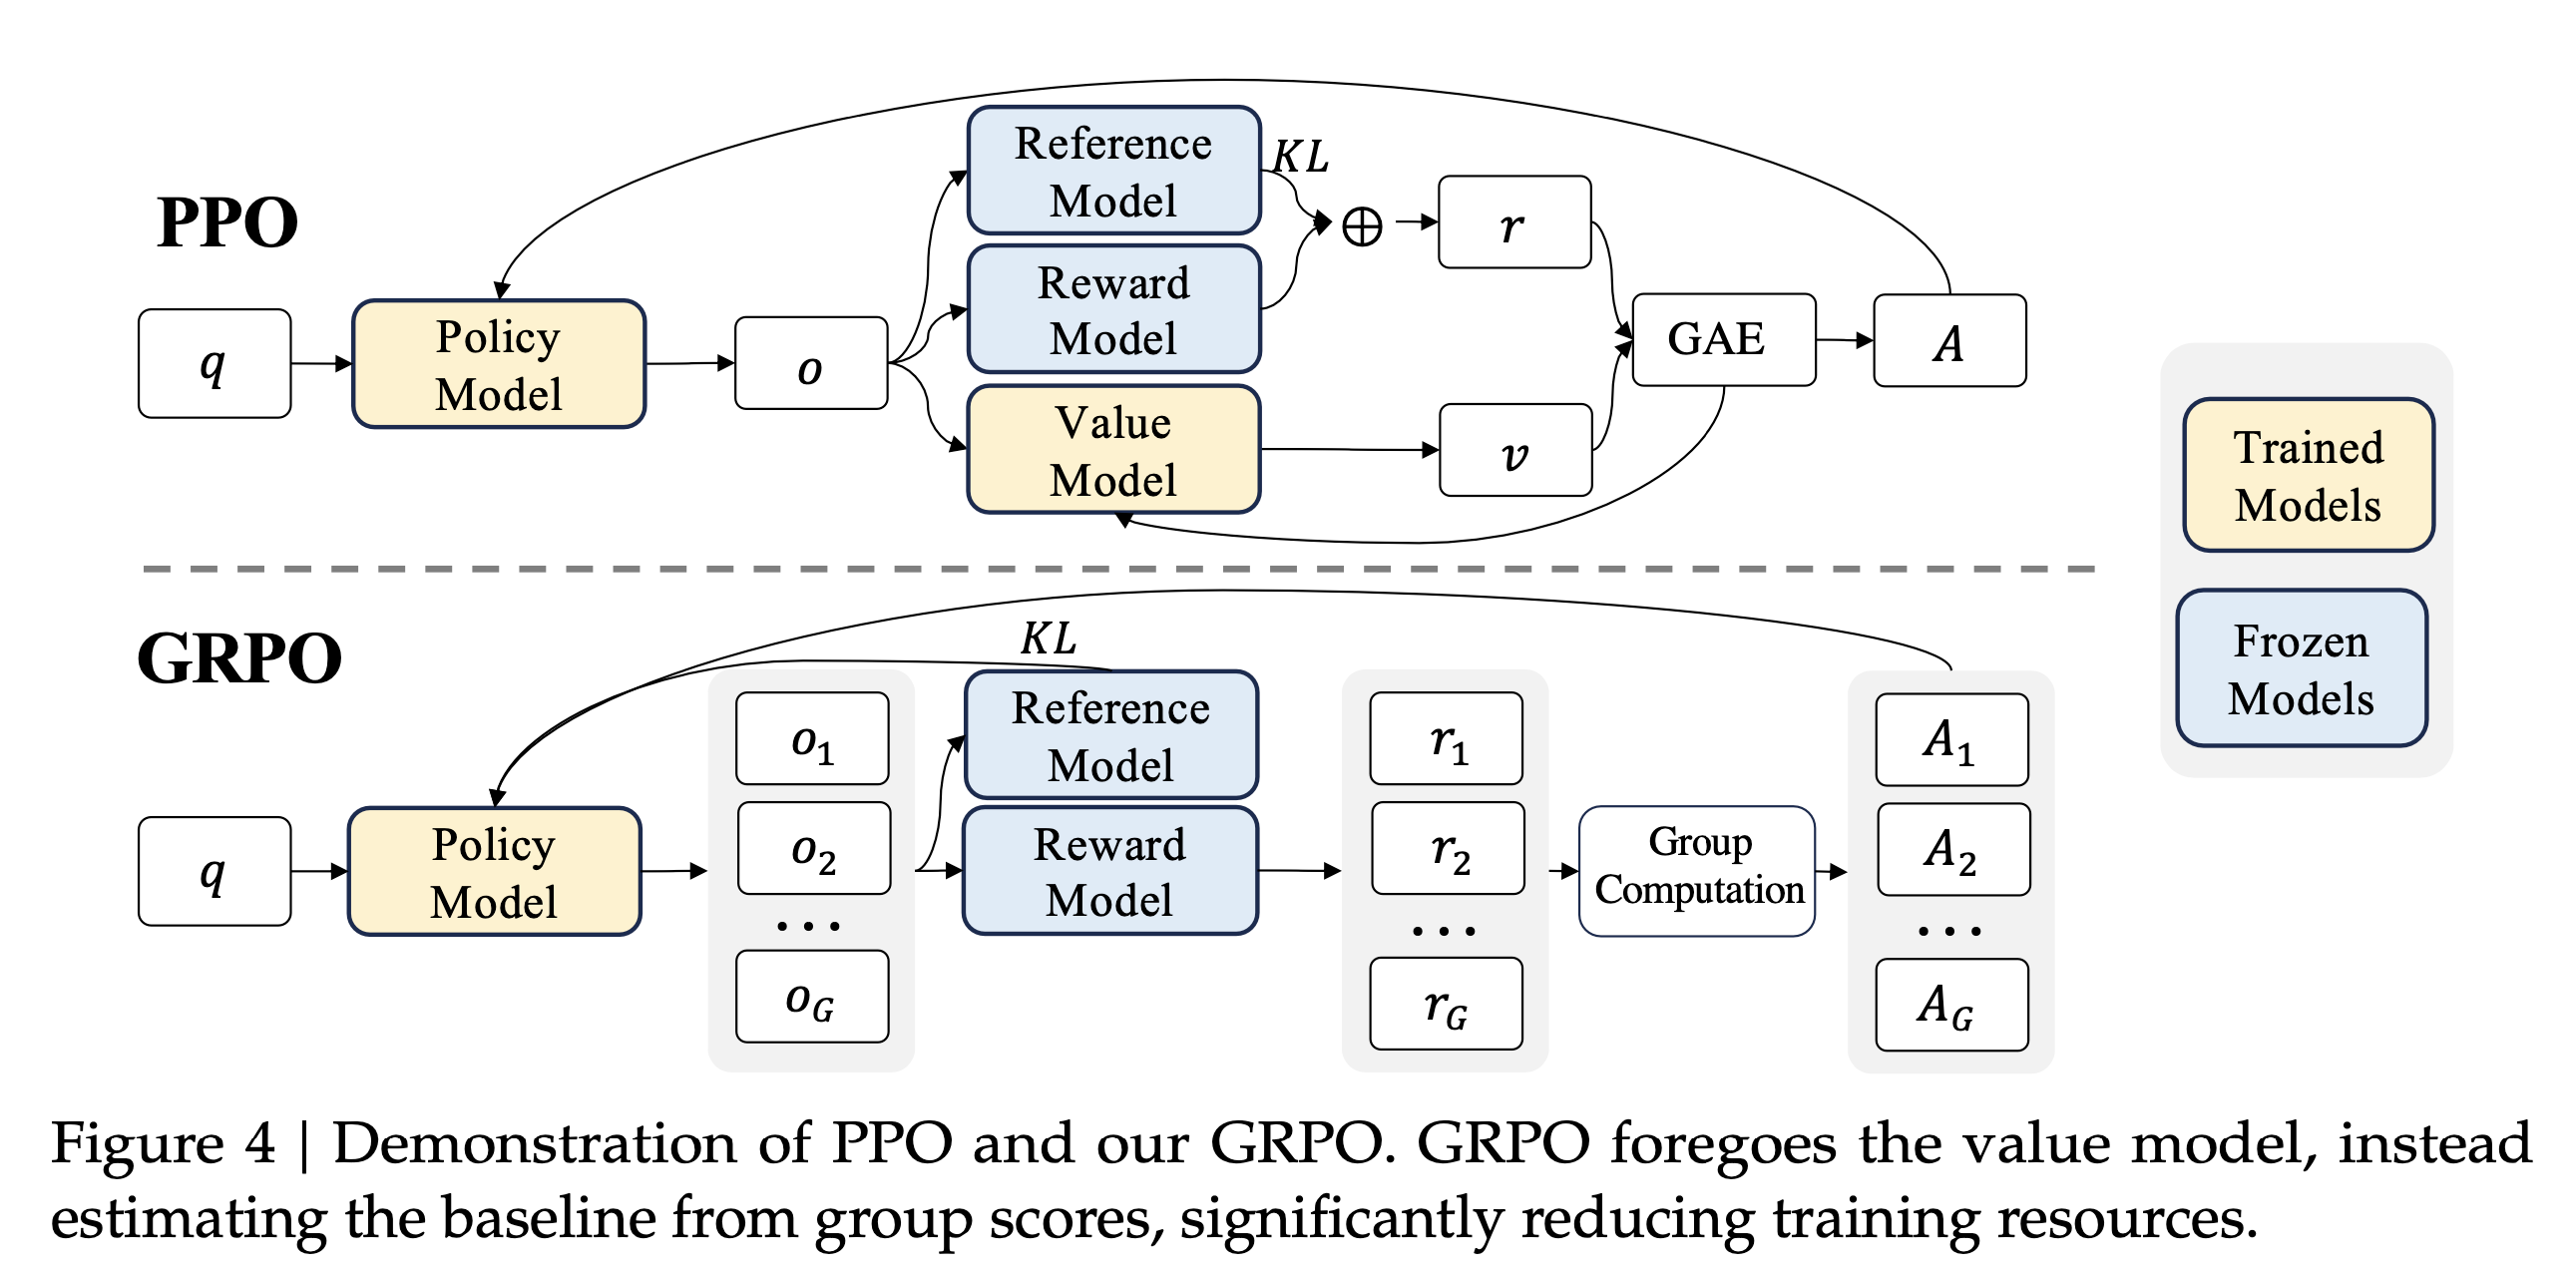
\includegraphics[width=1.0\textwidth]{figures/ppo_vs_grpo.png}
    \caption{PPO and GRPO diagram from \cite{shao2024deepseekmathpushinglimitsmathematical}.}
    \label{fig:trl2}
  \end{figure}

    \pause
  \begin{itemize}
  \item \textbf{No Value Model => significantly reduced training resources compared to PPO.}
\end{itemize}

\end{frame}


\begin{frame}{Iterative GRPO – Pseudocode}
  \begin{figure}
    \centering
    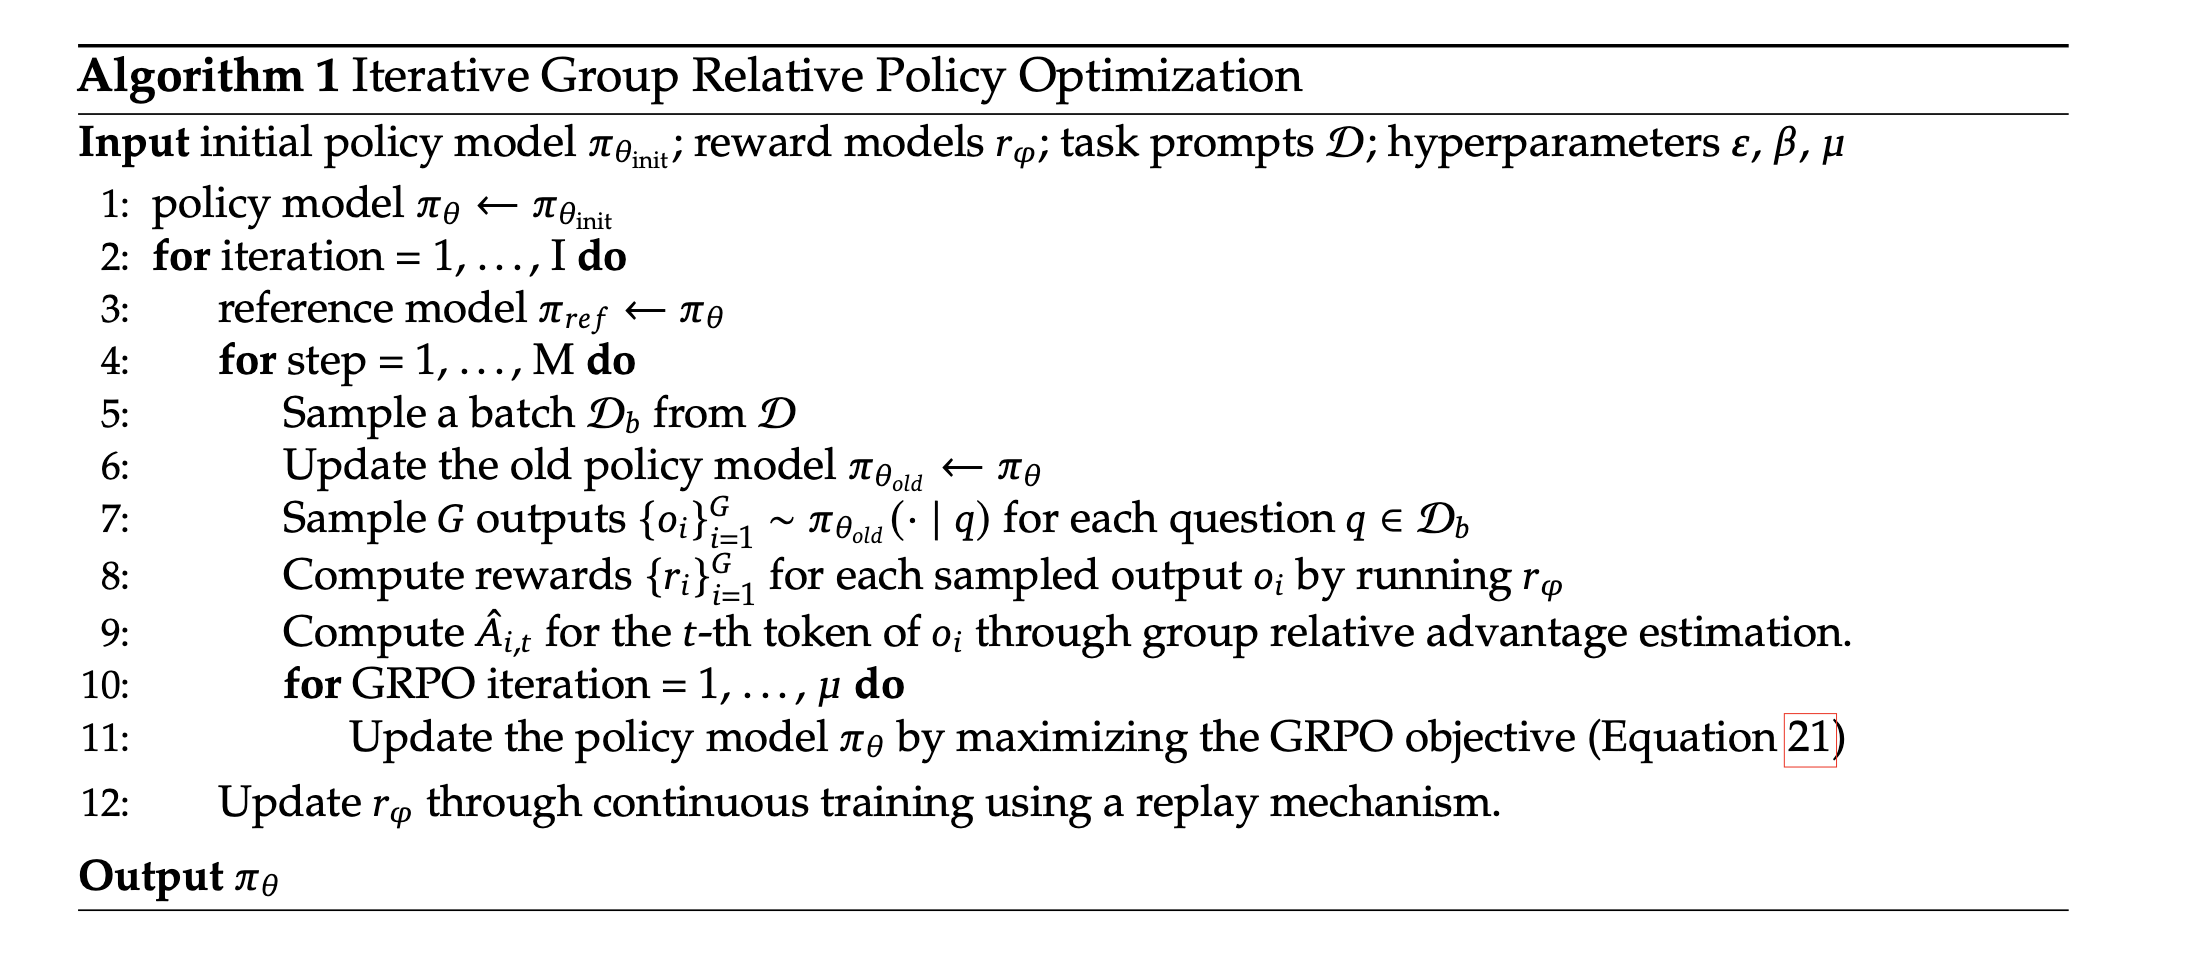
\includegraphics[width=1.0\textwidth]{figures/grpo_code.png}
    \caption{Iterative GRPO pseudocode from \cite{shao2024deepseekmathpushinglimitsmathematical}.}
    \label{fig:trl3}
  \end{figure}

\end{frame}

%–––––––––– Slide 1 ––––––––––%
\begin{frame}{DeepSeekMath}

\begin{itemize}\setlength\itemsep{0.3em}
  \item First paper to introduce GRPO for RL fine-tuning of an LLM.
  \vspace{0.5em}
  \item Specialized in mathematical reasoning and problem-solving.
\end{itemize}

\pause
\vfill
\textbf{Training pipeline:}
\begin{enumerate}

  \item Initialized with \textbf{DeepSeek-Coder-Base-v1.5 7B} \cite{guo2024deepseekcoderlargelanguagemodel}

  \vspace{0.5em}
  \item \textbf{Continued pre-training (unsupervised)}  
  \vspace{0.5em}
    \begin{itemize}
        \item Broad mathematical knowledge => \textbf{DeepSeekMath‑Base 7B}
    \end{itemize}

  \vspace{0.5em}
  \item \textbf{Supervised instruction fine-tuning (SFT)}  
    \begin{itemize}
        \item Prompt following and explicit reasoning => \textbf{DeepSeekMath‑Instruct 7B}
    \end{itemize}

  \vspace{0.5em}
  \item \textbf{GRPO reinforcement learning}  
    \begin{itemize}
        \item Improved reasoning capabilities => \textbf{DeepSeekMath‑RL 7B}
    \end{itemize}

\end{enumerate}\setlength\itemsep{0.45em}
\end{frame}


%----------------------------------------------------
\begin{frame}{Phase 1 – Continual Pre‑Training (DeepSeekMath‑Base)}
  \begin{block}{Motivation}
    DeepSeek‑Coder‑Base‑v1.5 lacked explicit mathematical domain knowledge.
  \end{block}
  \begin{itemize}
    \item \textbf{Data}: 500B tokens
    \begin{itemize}
        \item \textbf{56\% DeepSeekMath Corpus} (filtered Common Crawl)
        \item 4\% AlgebraicStack
        \item 10\% arXiv
        \item 20\% GitHub code
        \item 10\% CommonCrawl NL
    \end{itemize}
    \pause
    \vfill
    \item \textbf{Objective}: classical LM loss, maximize probability of next token prediction:
    $\displaystyle\mathcal L_{\text{LM}}=-\sum_t\log\pi_\theta(x_t\mid x_{<t})$
    \begin{itemize}
        \item “read the Internet and guess the next word”
    \end{itemize}
    \pause
    \vfill
    \item \textbf{Results}: Tops open‑source base models on GSM8K \& MATH, surpasses 540B Minerva (see in a couple of slides).
  \end{itemize}
\end{frame}

%----------------------------------------------------
\begin{frame}{Phase 2 – SFT (DeepSeekMath‑Instruct)}
  \begin{block}{Motivation}
    Base model not yet capable of instruction following or chain-of-thought.
  \end{block}
  \begin{itemize}
    \item \textbf{Data}: 776K problems (English \& Chinese) with
    \begin{itemize}
        \item 
          \textbf{CoT}: Natural-language reasoning steps.
        \item 
          \textbf{PoT}: Answer natural-language with python code that solves the task.
    \end{itemize}
    \vfill\pause
    \item \textbf{Objective}: Supervised cross-entropy on target answer: $\displaystyle\mathcal L_{\text{SFT}}=-\sum_{t=1}^{|o^\ast|} \log\pi_\theta(o^\ast_t\mid q,o^\ast_{<t})$
    \begin{itemize}
        \item $o^\ast$: gold solution written by human expert
        \item “write the expert answer I show you”
    \end{itemize}
    \vfill\pause
    \item \textbf{Results}: Beats all 7B peers and rivals 70B open‑source instruction‑tuned models (in two slides).
  \end{itemize}
\end{frame}

%----------------------------------------------------
\begin{frame}{Phase 3 – RL with GRPO (DeepSeekMath-RL)}
  \begin{block}{Motivation}
    Further align the model’s reasoning quality without relying on a value critic.
  \end{block}

  \begin{itemize}
    %----- DATA -----
    \item \textbf{Data}: 144K math prompts from \textbf{GSM8K} and \textbf{MATH}

        \vspace{0.8em}
    \pause
    %----- OBJECTIVE -----
    \item \textbf{Objective}: GRPO surrogate objective \eqref{eq:grpo_obj}
      \begin{itemize}
        \pause
        \item Reward model initialized from \textbf{DeepSeekMath-Base} -- with a scalar head attached, and fine-tuned on preference data.
        \pause
        \item For every prompt the policy samples a \textbf{64 candidate solutions ($G=64$)} to compute group relative advantage.
        \pause
        \item \textbf{Iterative GRPO outperforms a single-pass variant}
      \end{itemize}

        \vspace{0.8em}
    %----- OUTCOME -----
      \begin{figure}
        \centering
        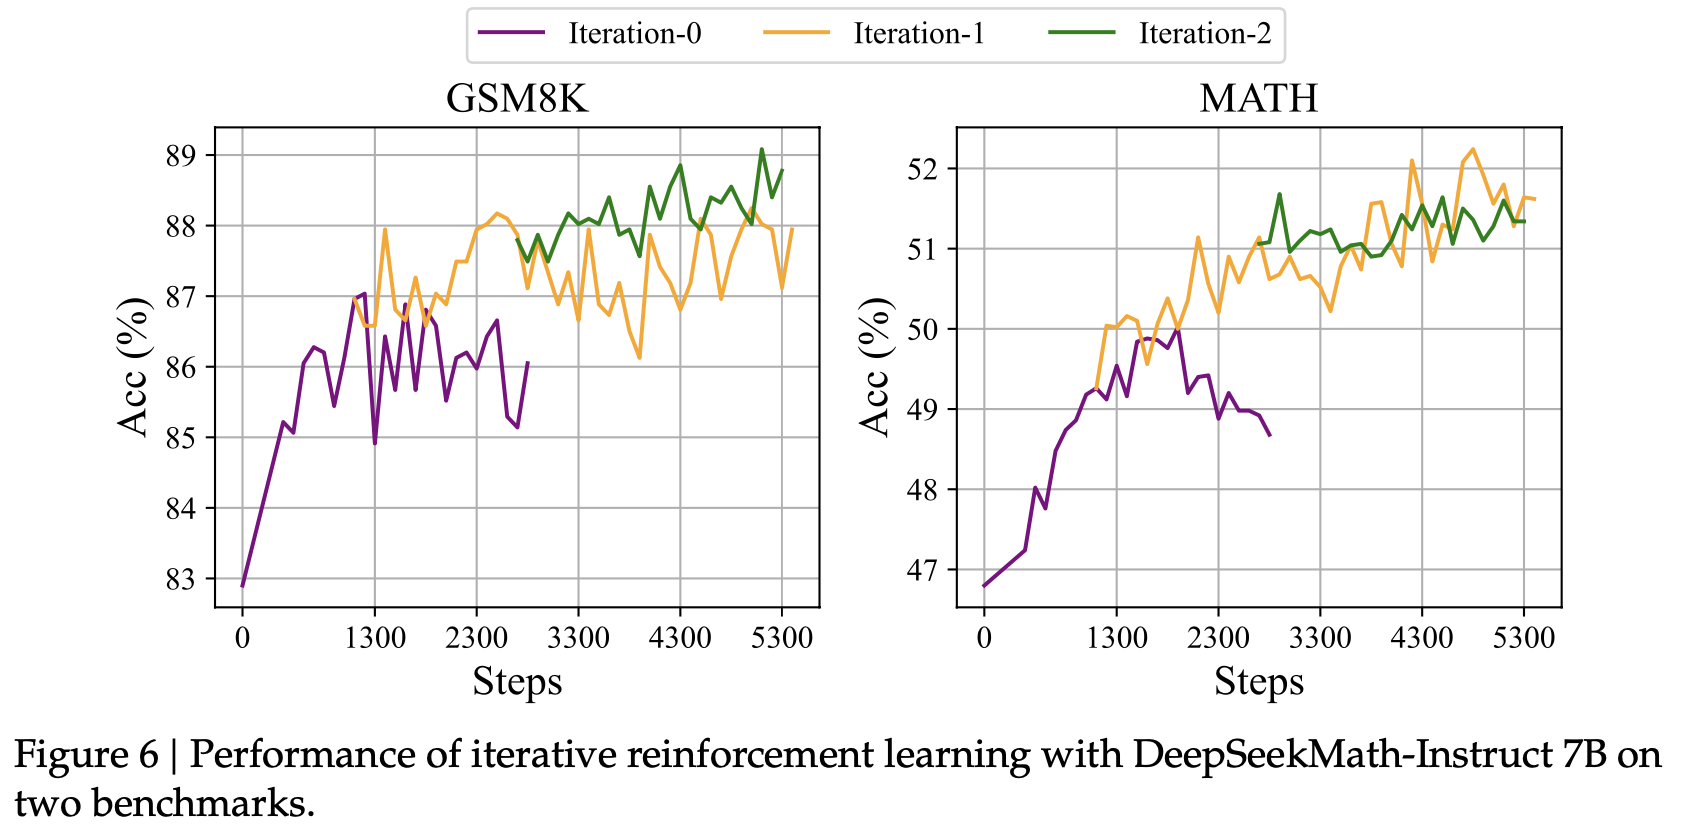
\includegraphics[width=0.6\textwidth]{figures/iterative.png}
        \caption{From \cite{shao2024deepseekmathpushinglimitsmathematical}.}
        \label{fig:trl4}
      \end{figure}
  \end{itemize}
\end{frame}



\begin{frame}{DeepSeekMath - Results}

  \begin{figure}
    \centering
    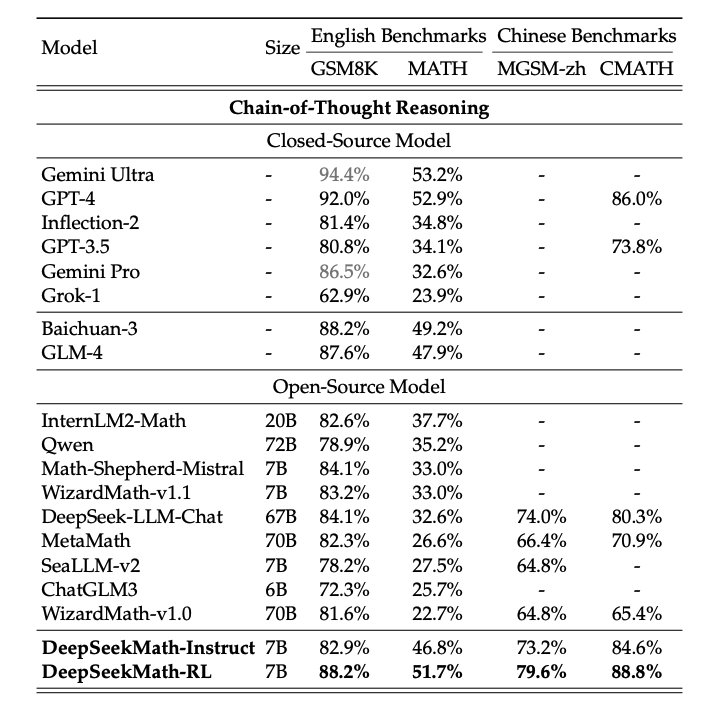
\includegraphics[width=0.6\textwidth]{figures/dsm_results.png}
    \caption{DeepSeekMath-RL 7B improves over DeepSeekMath-Instruct 7B and beats all open-source models from 7B to 70B, as well as the majority of closed-source models. From \cite{shao2024deepseekmathpushinglimitsmathematical}.}
    \label{fig:trl4_}
  \end{figure}

\end{frame}

\begin{frame}{DeepSeek-R1}

  \begin{figure}
    \centering
    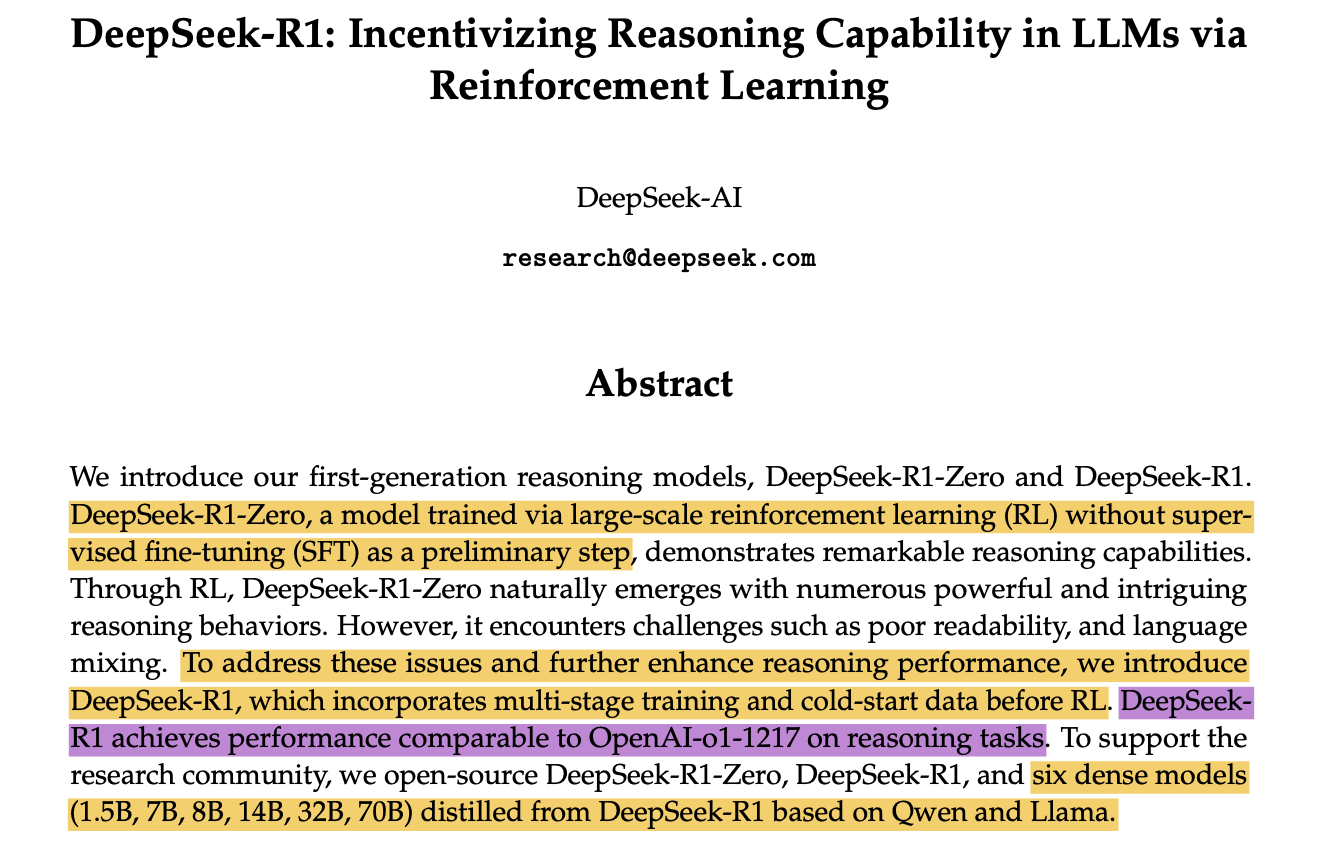
\includegraphics[width=0.8\textwidth]{figures/ds-r1.png}
    \label{fig:trl5}
  \end{figure}
  
\end{frame}


%–––––––––– DeepSeek-R1 overview ––––––––––%
\begin{frame}{DeepSeek-R1 overview}
\begin{itemize}\setlength\itemsep{0.35em}
  \item Introduced two reasoning models (671B): 
 \begin{itemize}
      \vspace{1em}
     \item \textbf{DeepSeek-R1-Zero} (pure RL with GRPO)
      \vspace{1em}
     \item \textbf{DeepSeek-R1} (multi-stage RL with GRPO + SFT)
 \end{itemize} 
      \vspace{1em}
\item And a family of distilled models based on \textbf{Qwen} \cite{qwen2025qwen25technicalreport} and \textbf{Llama} \cite{touvron2023llamaopenefficientfoundation} 1.5B-70B.
  \vspace{1em}
\pause
    \item Reaches \textbf{GPT-o1} level on math / code benchmarks
  \vspace{1em}
  \item Often mislabeled as "open-source"
  \begin{itemize}
      \item Model weights are open, the datasets and code used to train the model are not!
  \end{itemize}
\end{itemize}

\end{frame}

%–––––––––– R1-Zero stage ––––––––––%
\begin{frame}{DeepSeek-R1-Zero (pure RL with GRPO)}
\begin{itemize}\setlength\itemsep{0.35em}
  \item Initialized with \textbf{DeepSeek-V3-Base} \cite{deepseekai2025deepseekv3technicalreport}, only fine-tuned to reason with GRPO without any supervised data.
  \pause
  \vfill
  \item Reward model replaced with \textbf{rule based rewards}:
  \begin{itemize}
      \item \textbf{Accuracy rewards}: Response is correct (+1), i.e. math and code problems with deterministic results.
      \item \textbf{Format rewards}: Model is required to put its thinking process between <think></think> tags.
  \end{itemize}
  \vfill
  \begin{figure}
    \centering
    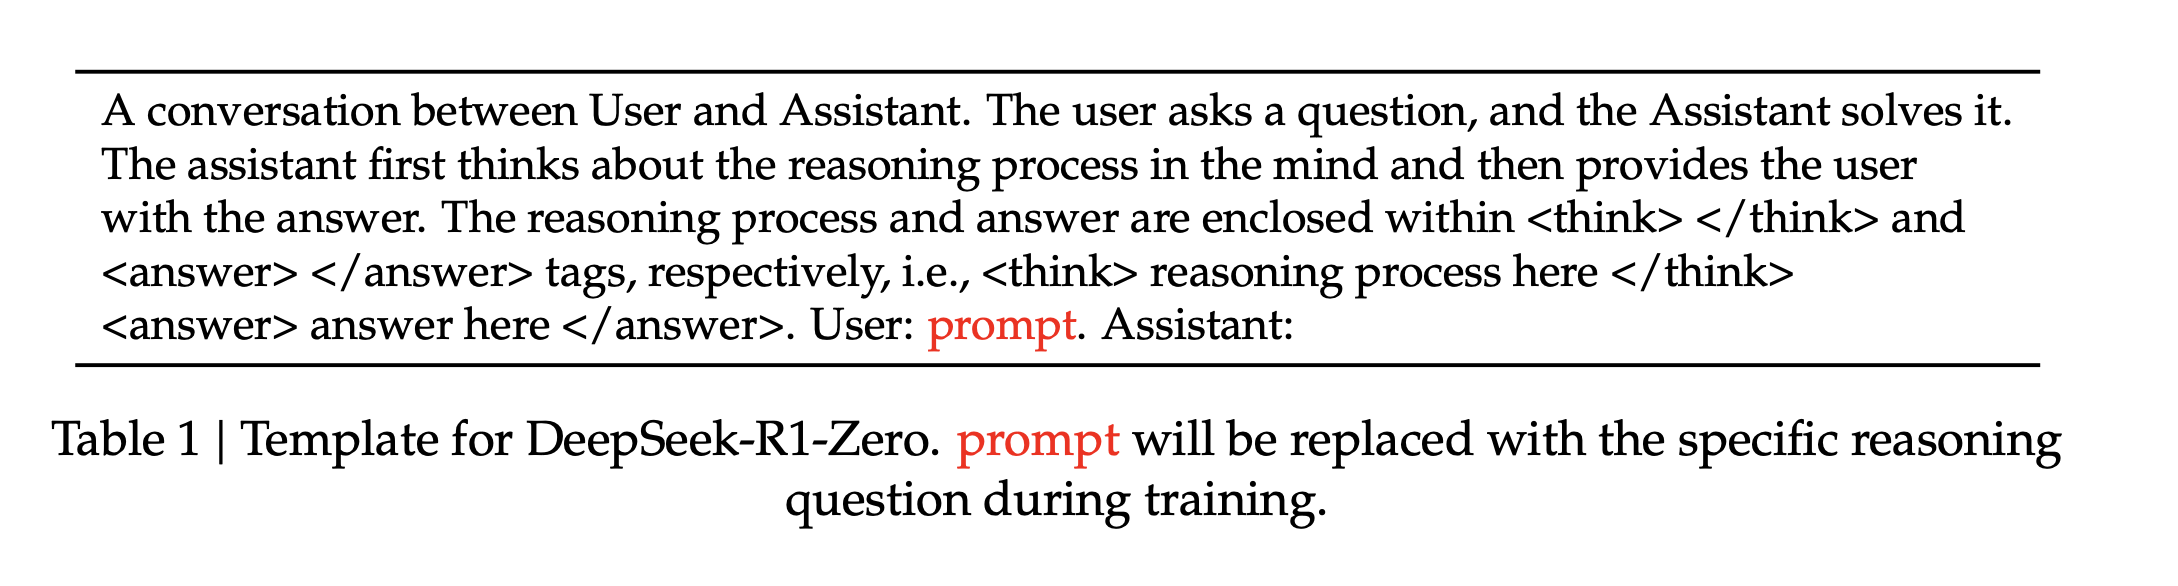
\includegraphics[width=0.8\textwidth]{figures/r1-zero-prompt.png}
    \caption{DeepSeek-R1-Zero training prompt, from \cite{deepseekai2025deepseekr1incentivizingreasoningcapability}.}
    \label{fig:trl6}
  \end{figure}
\end{itemize}
\end{frame}

\begin{frame}{DeepSeek-R1-Zero training -- Accuracy}

  \begin{figure}
    \centering
    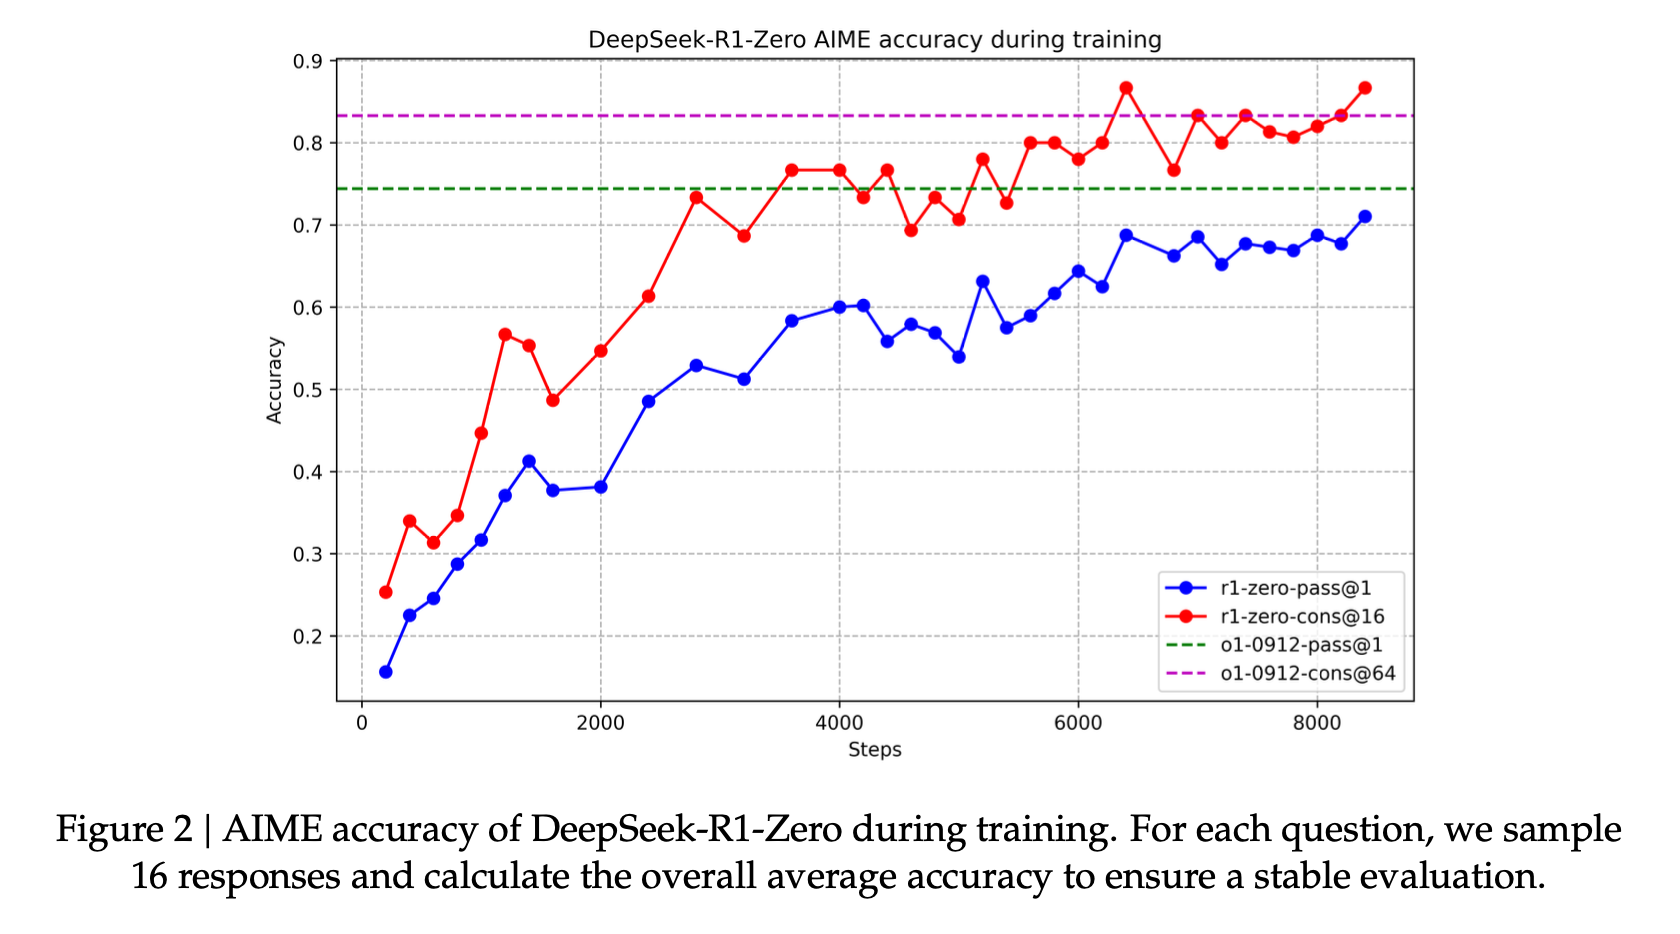
\includegraphics[width=0.8\textwidth]{figures/r1_zero_training.png}
    \caption{From \cite{deepseekai2025deepseekr1incentivizingreasoningcapability}.}
    \label{fig:trl7}
  \end{figure}
  
\end{frame}

\begin{frame}{DeepSeek-R1-Zero training -- Response length}

  \begin{figure}
    \centering
    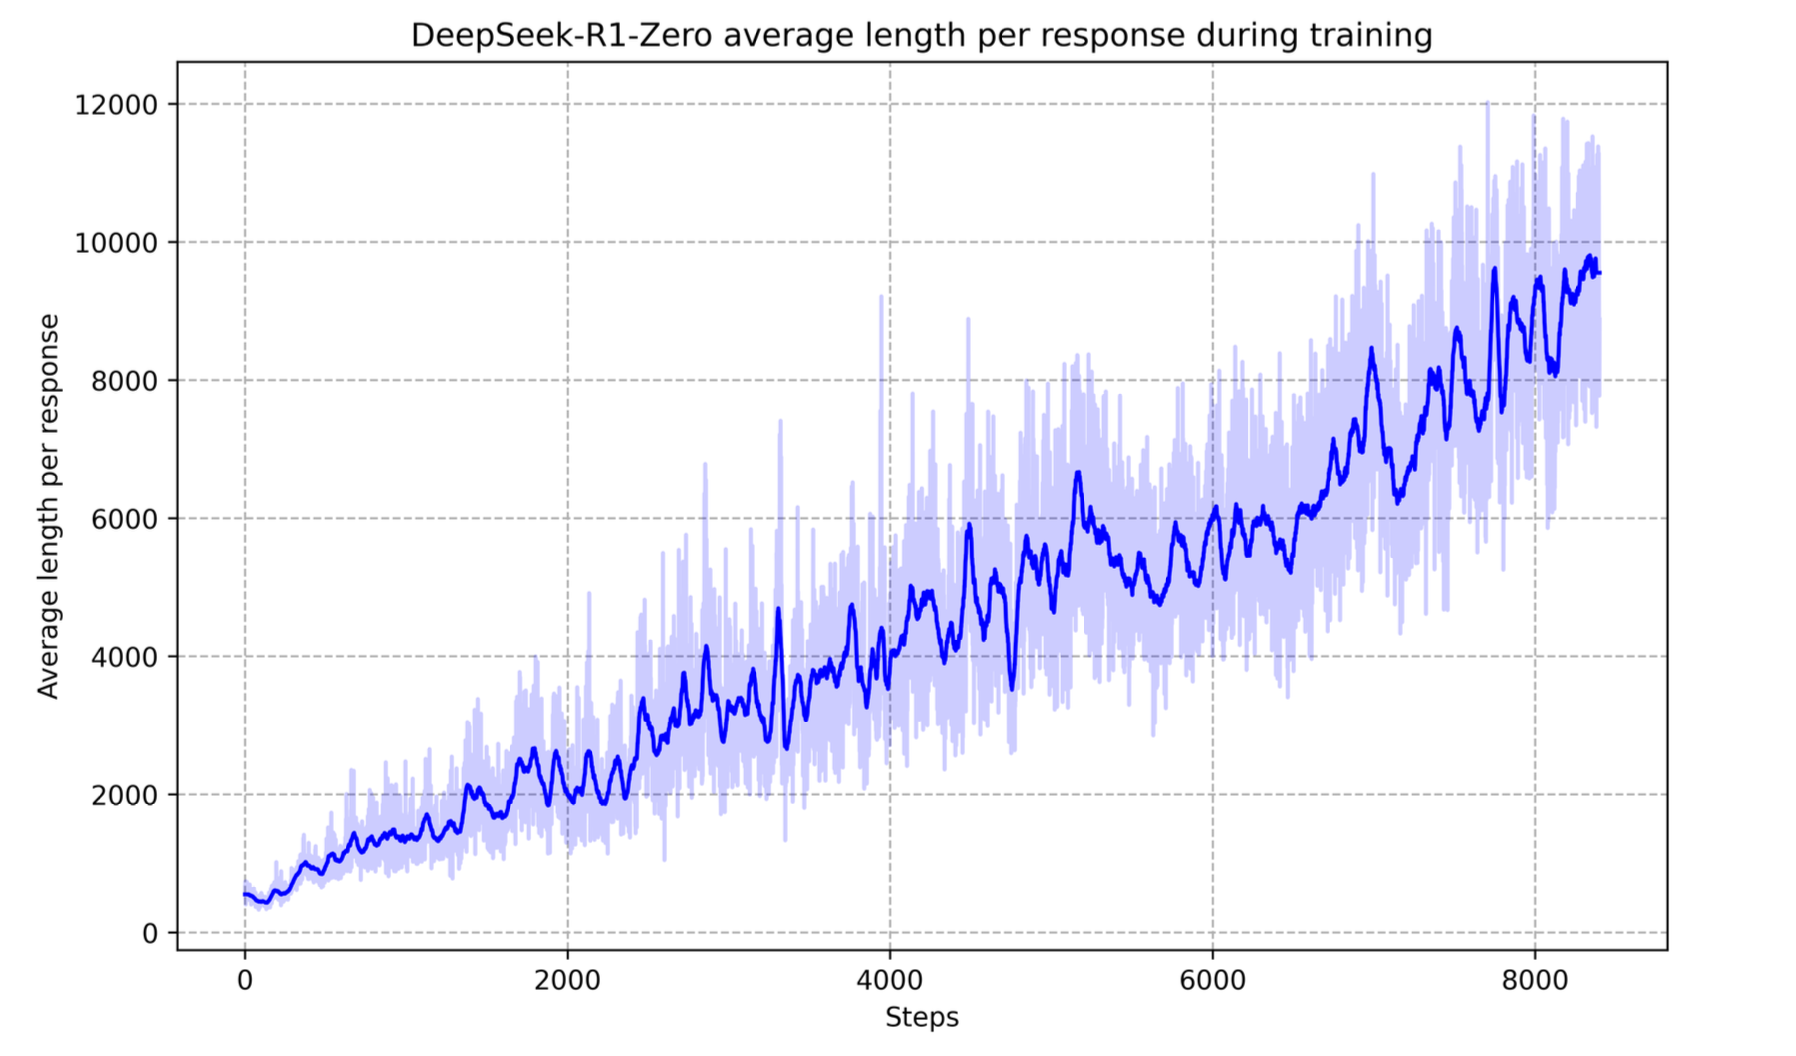
\includegraphics[width=0.8\textwidth]{figures/response-length.png}
    \caption{From \cite{deepseekai2025deepseekr1incentivizingreasoningcapability}.}
    \label{fig:trl8}
  \end{figure}

  \begin{itemize}
      \item "DeepSeek-R1-Zero naturally acquires the ability to solve increasingly complex reasoning tasks by leveraging extended test-time computation"
  \end{itemize}
  
\end{frame}

\begin{frame}{DeepSeek-R1-Zero training -- "Aha moment"}

  \begin{figure}
    \centering
    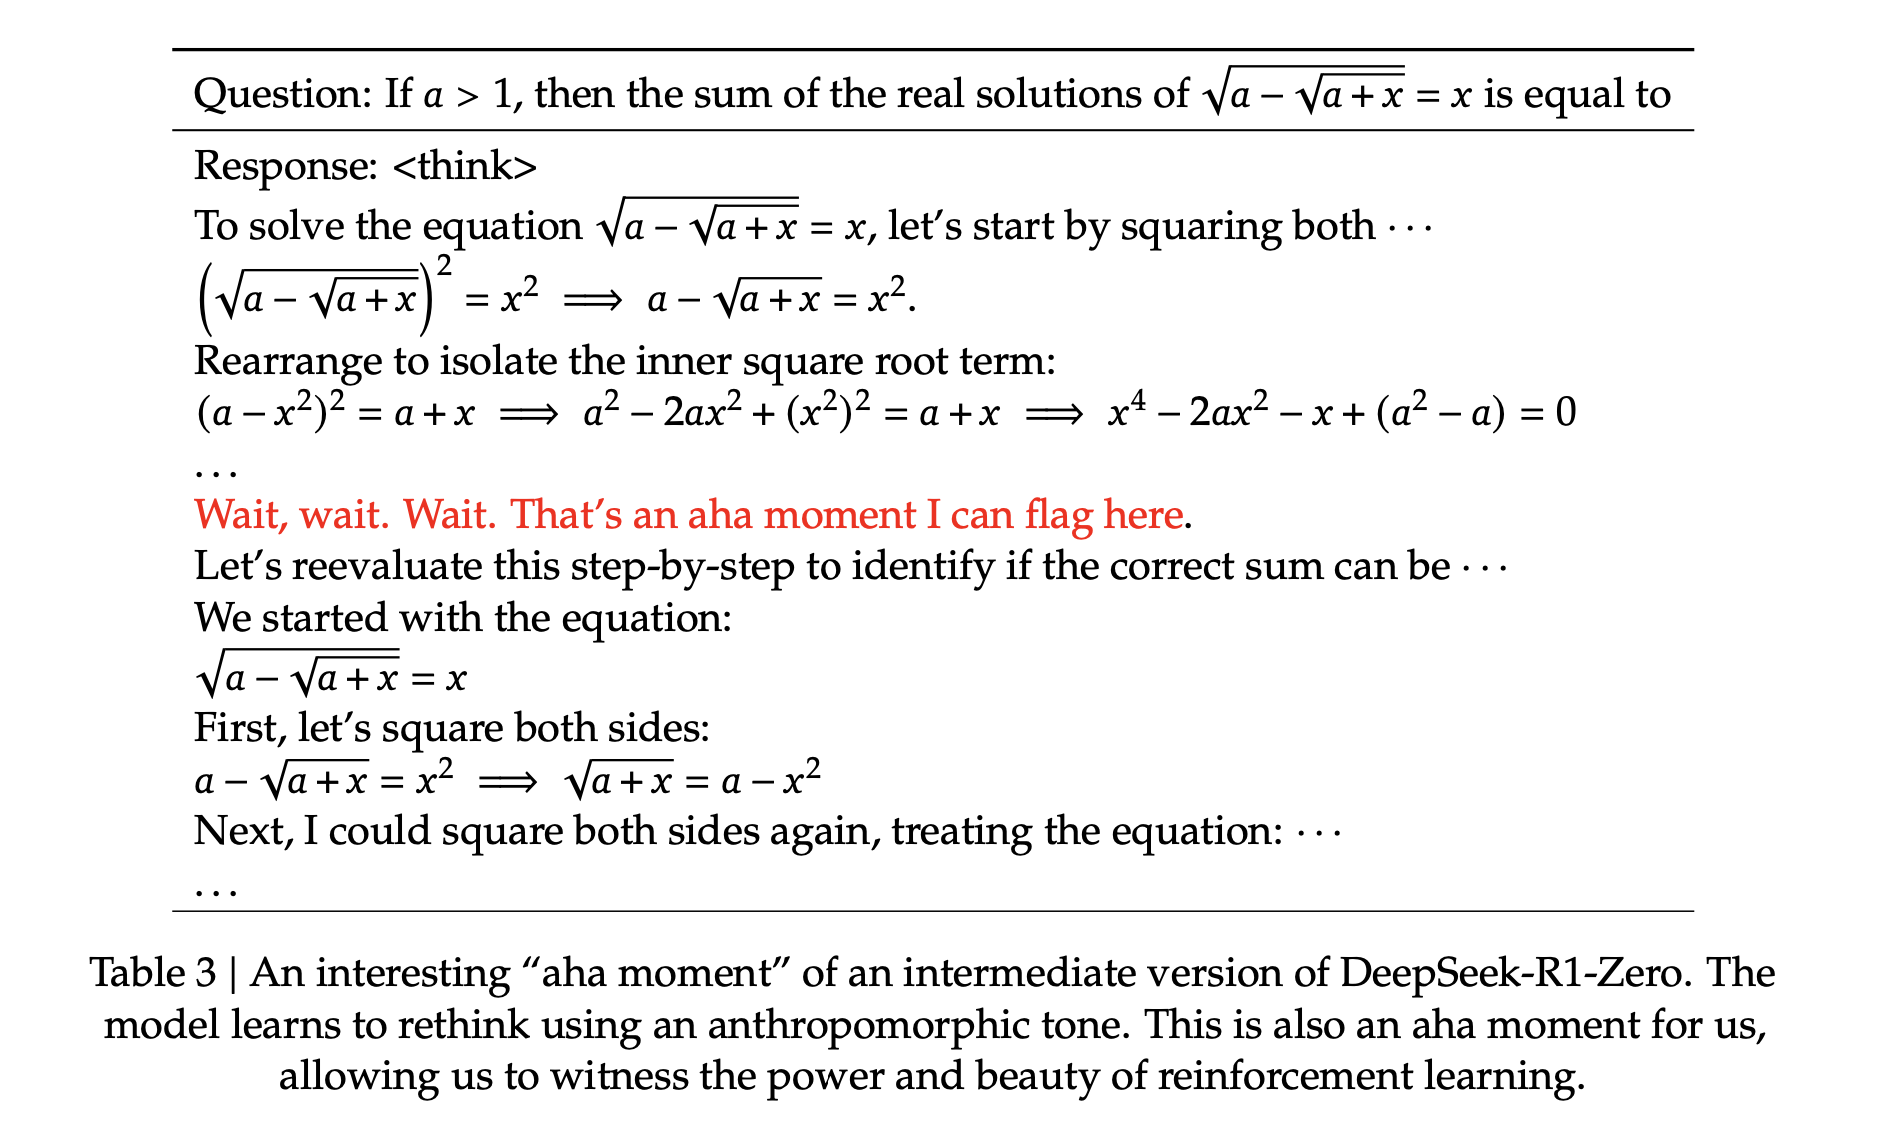
\includegraphics[width=0.9\textwidth]{figures/aha-moment.png}
    \caption{From \cite{deepseekai2025deepseekr1incentivizingreasoningcapability}.}
    \label{fig:trl9}
  \end{figure}

\begin{itemize}
    \item "DeepSeek-R1-Zero learns to allocate more thinking time to a problem by reevaluating its initial approach."
\end{itemize}
\end{frame}


%–––––––––– Full R1 pipeline ––––––––––%
\begin{frame}{DeepSeek-R1 –- Four-stage pipeline (SFT + GRPO)}
\begin{enumerate}\setlength\itemsep{0.4em}
\begin{block}{Motivation}
Problems with DeepSeek-R1-Zero: poor readability, language switching.
\end{block}
\pause
  \item \textbf{SFT}: finetune on thousands of curated CoT examples (exact data sources not released).
  \vspace{1.0em}
  \item \textbf{Reasoning-oriented RL with GRPO}: same rule-based rewards as R1-Zero + language-consistency rule (to prevent language switching).
  \pause
  \vspace{1.0em}
  \item \textbf{Rejection-sampling SFT}: \begin{itemize}
      \item 600K reasoning samples generated by model from previous stage. Filtered using rejection sampling (rule-based rewards for math \& code, DeepSeek-V3 judges equivalence with ground-truth for the rest).
      \vspace{0.5em}
      \pause
      \item 200K non-reasoning samples, e.g. factual QA, translation, "hello", ... (reused from DeepSeek-V3 pipeline).
  \end{itemize}
  \pause
  \vspace{1.0em}
  \item \textbf{RL with GRPO for all scenarios}: rule-based rewards for reasoning, helpful/harmless neural Reward Models for general queries
\end{enumerate}

\end{frame}

\begin{frame}{DeepSeek-R1 Results}

  \begin{figure}
    \centering
    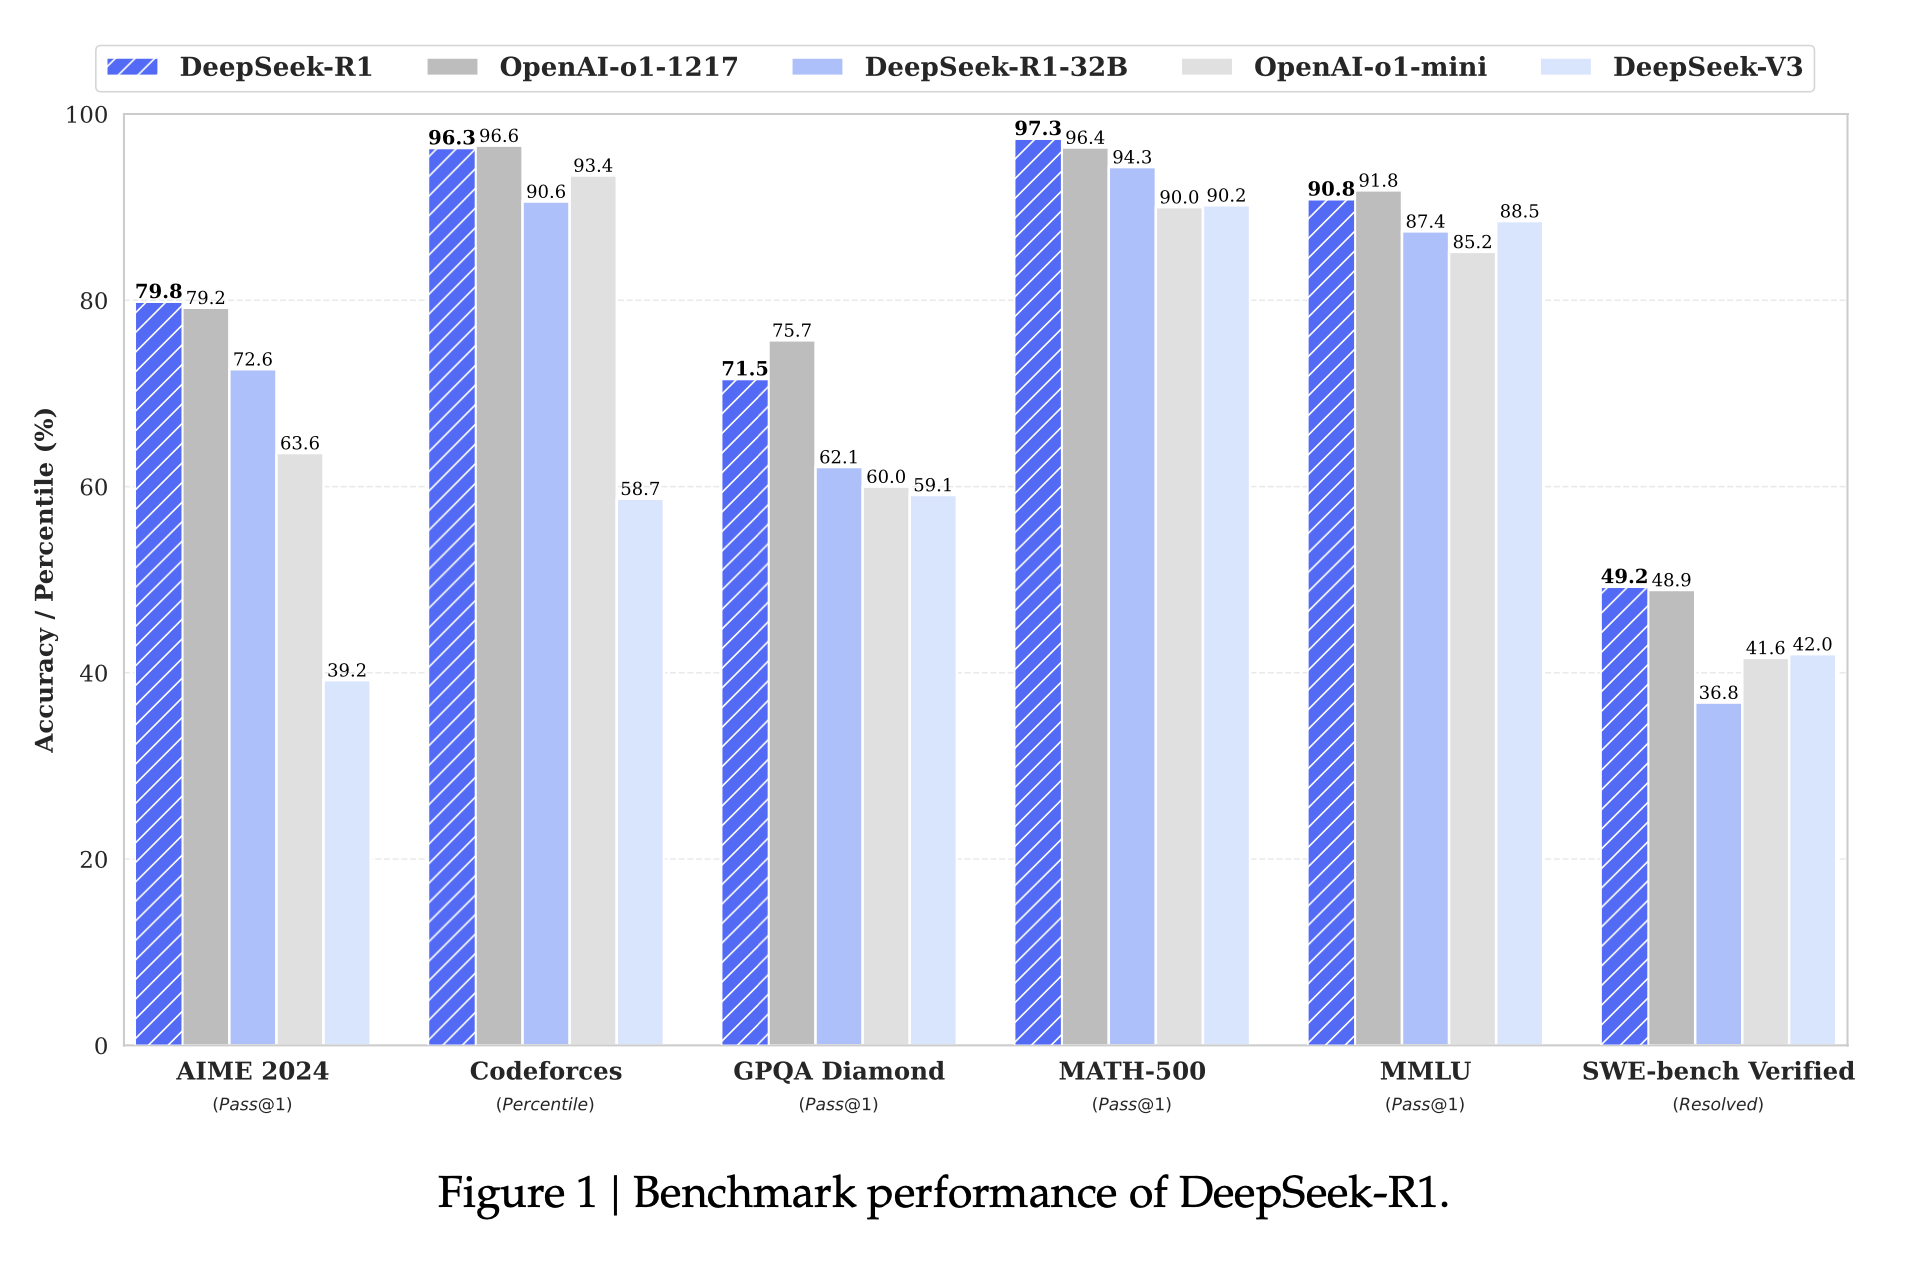
\includegraphics[width=0.9\textwidth]{figures/r1-results.png}
    \caption{From \cite{deepseekai2025deepseekr1incentivizingreasoningcapability}.}
    \label{fig:trl10}
  \end{figure}
  
\end{frame}


\begin{frame}{DeepSeek-R1-Distill Models}

\begin{itemize}
    \item Models from \textbf{Qwen} and \textbf{Llama} family trained by SFT with reasoning samples generated by \textbf{DeepSeek-R1}.
\end{itemize}

  \begin{figure}
    \centering
    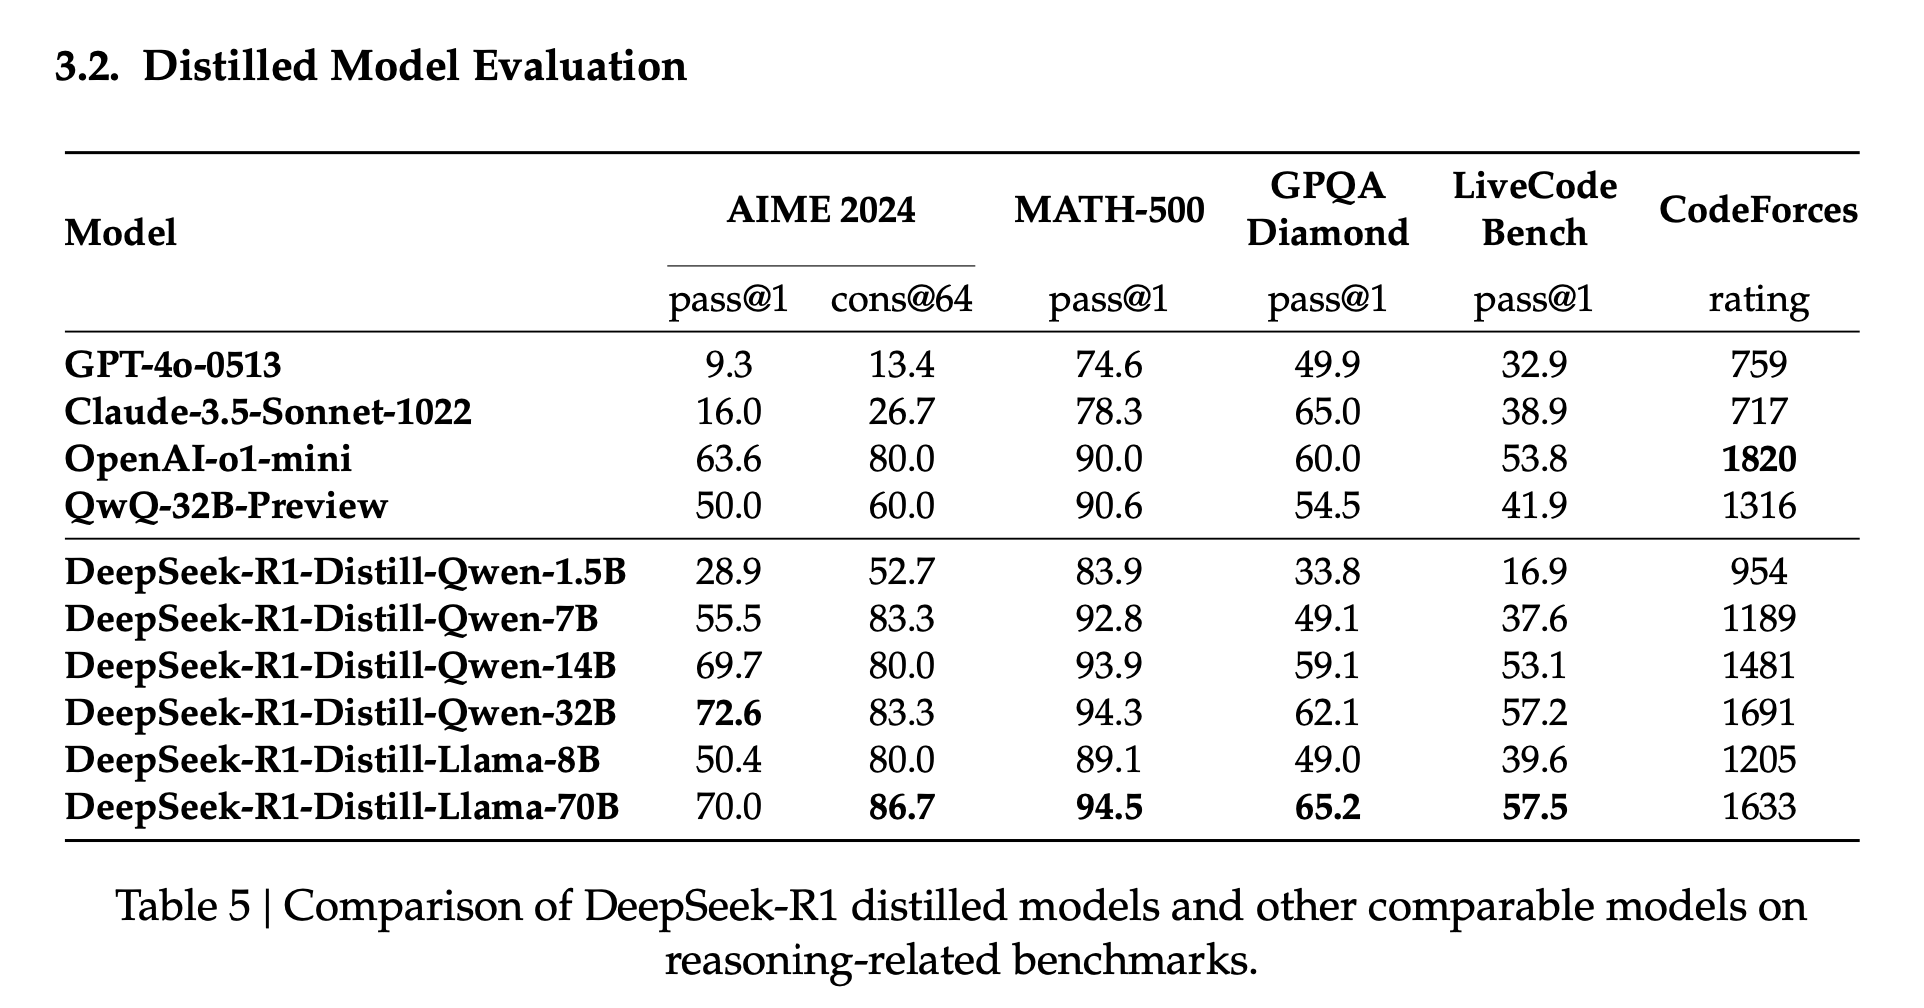
\includegraphics[width=0.9\textwidth]{figures/distill-eval-1.png}
    \caption{From \cite{deepseekai2025deepseekr1incentivizingreasoningcapability}.}
    \label{fig:trl11}
  \end{figure}
  
\end{frame}

\begin{frame}{DeepSeek-R1-Distill Models II}

\begin{itemize}
    \item \textbf{Interesting finding:} Applying large-scale RL on \textbf{Qwen-32B-Base} in the same way \textbf{DeepSeek-R1-Zero} was trained (10K steps) results in worse performance than SFT distillation!
\end{itemize}
  \begin{figure}
    \centering
    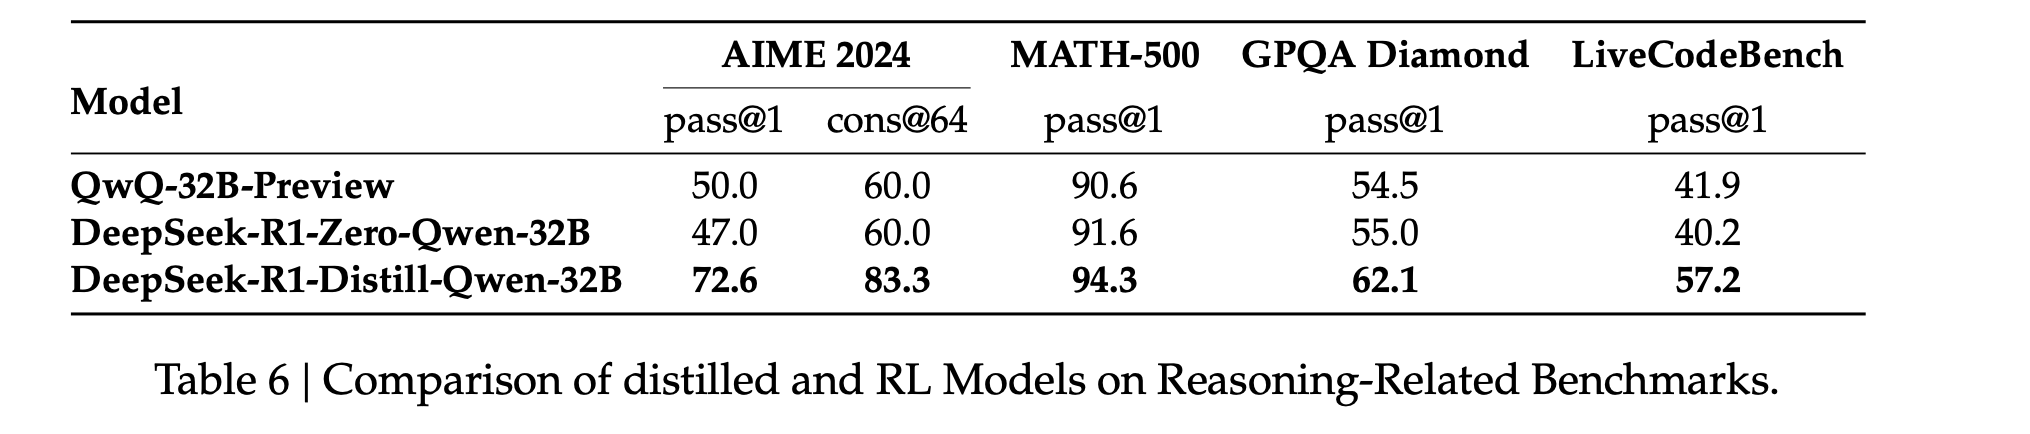
\includegraphics[width=0.9\textwidth]{figures/distill-eval-2.png}
    \caption{From \cite{deepseekai2025deepseekr1incentivizingreasoningcapability}.}
    \label{fig:trl12}
  \end{figure}
  
\end{frame}

\begin{frame}{Takeaways}

To train a strong reasoning model:
\vspace{1em}
\begin{itemize}
    \item You might not need a Value Model.
    \pause
    \vspace{1em}
    \item You might (sometimes) not even need a Reward Model.
    \pause
    \vspace{1em}
    \item You still need lot of engineering hacks (?)
      \begin{figure}
    \centering
    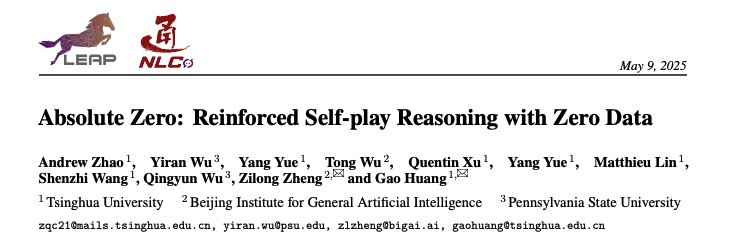
\includegraphics[width=0.9\textwidth]{figures/azr.png}
    \label{fig:trl13}
  \end{figure}
\end{itemize}

\end{frame}

\begin{frame}[t, allowframebreaks]{References}
\printbibliography[heading=none]
\end{frame}

\makeoutro

\end{document}